We now present a mobility pattern analysis for various population levels. Our dataset reveals mobility trends similar to those of CDRs (\S\ref{sec:mobility-patterns}) and generally represents the adjusted Census population well (\S\ref{sec:demographic-patterns}). In many cases we are able to detect differences in mobility patterns between ethnic groups and genders that can be plausibly explained by previous sociological findings (\S\ref{sec:mobility-patterns-by-Demographic}), and we are also able to detect segregation among ethnic groups (\S\ref{sec:ethnic-segregation}).

\subsection{Mobility Patterns}
\label{sec:mobility-patterns}

In order to compare the mobility patterns of our dataset to those in the CDR dataset of~\cite{Isaacman:2011cn,Isaacman:2010en} we only consider checkins for the years 2011 through 2013 each for the Spring months from March 15 to May 15 and for the Winter months from November 15 to January 31 (the LA and NY Spring and Winter subsets, respectively). Table \ref{tab:basics} shows the distribution of the data in our subsets compared to those in the CDR dataset~\cite{Isaacman:2011cn}. The mobility traces from our subsets are much more sparse. Most notably, while the CDR dataset has at least eight location points from call activity per day for the median user in LA and NY---and even 12 if text messages are added---the data in all of our subsets account for only one location point for the median user per day.

\begin{table}[t]
\centering
{\small
\begin{tabular}{| l | c | c | c | c | c | c | c |}
\hline
 & \multicolumn{2}{c|}{\textit{Spring}}& \multicolumn{2}{c|}{\textit{Winter}}  \\ \hline
\textit{Statistic} & LA          & NY           & LA          & NY \\ \hline
Total Checkins     & 135,503     & 109,506      & 118,446     & 98,286  \\
(Total CDRs)       & (74M)       & (62M)        & (247M)      & (161M) \\ \hline
Min. Loc./Day      & 1           & 1            & 1           & 1 \\ \hline
1st Qu. Loc./Day   & 1           & 1            & 1           & 1 \\ \hline
Med. Loc./Day      & \textbf{1}  & \textbf{1}   & \textbf{1}  & \textbf{1} \\
(Med. Calls/Day)   & \textbf{(9)}& \textbf{(10)}& \textbf{(8)}& \textbf{(9)} \\ 
(Med. Texts/Day)   & -           &  -           & \textbf{(4)}& \textbf{(3)} \\ \hline
Mean Loc./Day      & 1.97        & 2.12         & 1.96        & 2.1 \\ \hline
3rd Qu. Loc./Day   & 2           & 2            & 2           & 2 \\ \hline
Max Loc./Day       & 73          & 62           & 98          & 69 \\ \hline		
\end{tabular}
}
\caption{Statistics of our LA and NY subsets compared to the CDR dataset in~\protect\cite{Isaacman:2011cn} (where available, in parentheses). Our calculations do not consider any day where a user had no checkins.}
\label{tab:basics}
\end{table}

Another insightful metric for comparing mobility patterns is the \emph{daily range}, defined as the maximum straight line distance a phone has traveled in a single day~\cite{Isaacman:2010en}. Daily ranges are characteristic for mobility because, for example, median daily ranges on weekdays represent a lower bound for a commute between home and work locations~\cite{Isaacman:2010en}. Figure~\ref{fig:ranges} shows a subset of our results. Our ranges are generally smaller than those reported by~\cite{Isaacman:2011cn,Isaacman:2010en}. However, the general trends in both datasets are similar. Most importantly, people in LA have generally greater ranges than people in NY. Also, in both areas people tend to travel longer during the day than at night. However, there are also differences: according to our data New Yorkers in the 98th percentiles travel farther than Angelinos.

\begin{figure}[t]
	\centering
	\begin{subfigure}[t]{1in}
		\centering
		\includegraphics[width=1in]{fig/footprints/max_ranges.eps}
    % \includegraphics[width=1in]{fig/max_ranges.eps}
	\end{subfigure}
	\begin{subfigure}[t]{1in}
		\centering
    \includegraphics[width=1in]{fig/footprints/med_ranges_day.eps}
		% \includegraphics[width=1in]{fig/med_ranges_day.eps}
	\end{subfigure}
	\begin{subfigure}[t]{1in}
		\centering
    \includegraphics[width=1in]{fig/footprints/med_ranges_night.eps}
		% \includegraphics[width=1in]{fig/med_ranges_night.eps}
	\end{subfigure}
	\vspace{2ex}

	{\small
\begin{tabular}{| l | c | c | c | c | c | c | c | c | c |}
\hline
           & \multicolumn{2}{c|}{\textit{Max. Mo.--Fr.}} & \multicolumn{2}{c|}{\textit{Med. Mo.--Fr.}} & \multicolumn{2}{c|}{\textit{Med. Night}}  \\ \hline
\%       & LA       & NY       & LA      & NY      & LA      & NY \\ \hline
98       & 2,471.7  & 3,625.6  & 133     & 209.9   & 117.4   & 129.9 \\
         & (2,467)  & (2,455)  & (32)    & (29)    & (23.1)  & (19.4) \\ \hline
75       & 47.5     & 37       & 9.3     & 5.3     & 6.1     & 3.3 \\
         & (130)    & (111)    & (10)    & (8.2)   & (8)     & (5.6) \\ \hline
50       & \textbf{12.8}     & \textbf{8.1}        & \textbf{4}   & \textbf{2.2}   & \textbf{1.6}   & \textbf{1} \\
         & (36)     & (27)     & (5)     & (3.8)   & (4)     & (2.6) \\ \hline
25       & 3        & 2.3      & 0.8     & 0.5     & 0.1     & 0.1 \\
         & (17)     & (12)     & (2)     & (1.3)   & (1.4)   & (0.7)\\ \hline
02       & $\epsilon$ & $\epsilon$ & $\epsilon$& $\epsilon$& $\epsilon$& $\epsilon$ \\
         & (1.6)    & (1.3)    & (0)   & (0)   & (0)   & (0)\\ \hline
\end{tabular}
}
	\caption{Daily ranges in miles. Top: boxes show the 25th, 50th, and 75th percentiles; whiskers the 2nd and 98th percentiles. Bottom: table with the percentiles represented in the boxplots. The maximum range (Max. Mo.--Fr.) is a user's longest distance and the median range (Med. Mo.--Fr.) a user's median distance, each taken on a single day for the entire Spring subset on a weekday~\protect\cite{Isaacman:2010en}. The median range at night (Med. Night) represents the median distance a user has traveled on a day for the entire combined Spring and Fall subset from 7pm--7am ~\protect\cite{Isaacman:2011cn}. Previous results~\protect\cite{Isaacman:2011cn,Isaacman:2010en} are shown in parentheses. Our calculations do not consider any day where a user had a zero range, that is, had multiple checkins at the same location or a single checkin only. We define $\epsilon<0.005$ miles.}
\label{fig:ranges}
\end{figure}

\subsection{Demographic Patterns}
\label{sec:demographic-patterns}

As our LA and NY subsets are annotated with ethnicity and gender labels (\S\ref{sec:method}) we are able to compare the resulting demographic distributions to the respective Census distributions. However, initial comparisons reveal substantial differences. For example, according to the Census there are more females than males (53\% vs. 47\%) living in Kings County~\cite{census:2010} while our observed label frequencies suggest that there should be substantially fewer (43\% vs. 57\%). This result is even more surprising as the gender-specific usage rates of Internet (70\% vs. 69\%)~\cite{file:2013} and Instagram (16\% vs. 10\%)~\cite{Pew2012} should further increase the percentage of females beyond the Census. However, while 86\% of female social network account owners set their profile to private, only 74\% of males do so~\cite{PewSocialMedia2012}. Adjusting the Census distribution for this difference (as well as for gender-specific Internet and Instagram usage rates) leads to a distribution of females and males (49\% vs. 51\%) much closer to the distribution we observed for our labels.

Similarly to gender, we make adjustments to the Census distributions for the varying percentages of Internet and Instagram usage rates among different ethnicities as well. However, even then we still observed a substantial Hispanic underrepresentation, which was also observed for the southwest of the United States by~\cite{mislove-2011-twitter}. We found this phenomenon difficult to assess, specifically, as ethnicity is not significant for setting a profile private~\cite{journals/jcmc/LewisKC08}, activity levels (posting pictures, etc.) are not lower for Hispanics~\cite{statista}, and our annotation disagreements are not higher when the Hispanic label is involved. However, we believe that the reason for the underrepresentation is the perception of Caucasian Hispanics as Caucasian alone. In a study, six of seven Caucasian Hispanics reported that others see them as Caucasian alone~\cite{MelaninMillennium}. Therefore, we believe that most Caucasian Hispanics were actually labeled as Caucasian (i.e., our annotators agreed on an incorrect classification). Thus, we adjusted the observed label frequencies by adding to the Hispanic labels a number of labels corresponding to the Census percentage of Caucasian Hispanics and subtracting the same number from the Caucasian labels.

\begin{figure}[t]
  \centering
  \includegraphics[width=3.35in]{fig/footprints/map.jpg}
	\vspace{0.2ex}

{\small
\begin{tabular}{| l | c | c | c | c | c |}
\hline
 & \multicolumn{2}{c|}{\textit{Ethnicity Multi-Cat.}} & \multicolumn{2}{c|}{\textit{Ethnicity Binary}} & \textit{Gender}  \\ \hline
\textit{Gran.} & LA       & NY                & LA      & NY                              & NY \\ \hline
State          & 0/1      & 0/1               & 1/1     & 0/1                             & 1/1 \\
               & (0\%)    & (0\%)             & (100\%) & (0\%)                           & (100\%) \\ \hline
County         & 1/2      & \textbf{8/11}     & 2/2     & 6/8                             & 4/4 \\
               & (50\%)   & \textbf{(73\%)}   & (100\%) & (75\%)                          & (100\%) \\ \hline 
PUMA           & 12/16    & 11/17             & 2/2     & 5/6                             & 1/1\\ 
               & (75\%)   & (65\%)            & (100\%) & (83\%)                          & (100\%) \\ \hline
NTA            & -        & 9/16             & -       & 7/7                             & 2/2\\
               & -        & (56\%)            & -       & (100\%)                         & (100\%) \\ \hline
ZIP            & 3/3      & 8/14              & 1/1     & 3/3                             & -  \\
               & (100\%)  & (57\%)            & (100\%) & (100\%)                         & - \\ \hline
\end{tabular}
}
\caption{Chi square goodness of fit test results for ethnicity and gender at various levels of Census-defined granularity. Top: detailed view of the multi-category ethnicity distributions for the NY county level. Left bars show the Census distributions (Cen.) and right bars the label distributions (Label). Bottom: complete results of the chi square tests. NTAs are specific to NY and not available for LA. Below the ZIP code and NTA levels we did not have enough data to perform chi square tests. We follow ~\protect\cite{Roscoe:1971} and require the average expected frequency for a chi square test with more than one degree of freedom to be at least two and for a test with one degree of freedom to be at least 7.5. To prevent skewing due to small sample sizes we also use a Monte Carlo simulation with 2,000 replicates.}
\label{fig:map}
\end{figure}

\begin{figure}[t]
	\centering
    \includegraphics[width=3.35in]{fig/footprints/max_ranges_eth_ny.eps}
		% \includegraphics[width=3.35in]{fig/max_ranges_eth_ny.eps}
    \includegraphics[width=3.35in]{fig/footprints/med_ranges_gender_ny.eps}
		% \includegraphics[width=3.35in]{fig/med_ranges_gender_ny.eps}
	\vspace{0.1ex}

{\small
\resizebox{\columnwidth}{!}{%
\begin{tabular} {| l | c | c | c | c | c | c |}
\hline
           & \multicolumn{4}{c|}{\textit{Max. Mo.-Fr. NY}} & \multicolumn{2}{c|}{\textit{Med. Night NY}}  \\ \hline
\%           & Hisp.   & Cauc.   & Af. A.  & Oth.    & Fem.  & Male \\ \hline
98           & 2,480.8 & 6,509.4 & 2,270.9 & 6,788.1 & 9.8   & 11.5 \\ \hline
75           & 50.8    & 592.3   & 44      & 187     & 3.2   & 4.7 \\ \hline 
50           & \textbf{13.5}    & \textbf{52.1}    & \textbf{11.9}    & \textbf{18.4}    & \textbf{1.8}   & \textbf{1.9} \\ \hline 
25           & 4.9     & 7       & 5.5     & 3.7     & 0.4   & 0.6 \\ \hline 
02           &$\epsilon$&$\epsilon$&$\epsilon$&$\epsilon$&$\epsilon$&$\epsilon$\\ \hline 
\end{tabular}
}}
	\caption{Daily ranges in miles. Top: density plot of the maximum daily ranges by ethnicity. Middle: density plot of the median daily ranges at night by gender. Bottom: table with the percentiles of the daily ranges represented in the plots. We rounded extremely small daily ranges up to 0.005 miles. Our calculations do not consider any day where a user had a zero range, that is, had multiple checkins at the same location or a single checkin only. We define $\epsilon<0.005$ miles.}
	\label{fig:ranges_ny}
\end{figure}

We perform chi square tests for goodness of fit comparing the gender and ethnicity distributions of our labels to the corresponding Census distributions for different levels of granularity. In most cases we obtain a value of $p>0.05$ and find no evidence to reject the null hypothesis that the observed gender and ethnicity distributions follow the corresponding Census distributions. For example, as shown in Figure~\ref{fig:map}, for eight out of 11 counties in the NY area our tests resulted in $p>0.05$ providing no evidence that our multi-category ethnicity distributions deviate significantly from the Census distributions. However, there are also cases with differences. It is no surprise that this is true for the state level as our distributions only cover users from the LA and NY metropolitan areas. However, overall we believe our results suggest that geotag data often replicate demographic trends faithfully.

\subsection{Mobility Patterns by Demographic}
\label{sec:mobility-patterns-by-Demographic}

By combining our methodologies from the previous two subsections we now show the differences in mobility patterns between ethnic groups and between males and females, respectively. In particular, we examine differences in daily ranges, home ranges, and temporal checkin characteristics.

\paragraph{Daily Ranges}

Figure~\ref{fig:ranges_ny} shows some of our daily range results for ethnic groups and genders based on our sets of labeled users for LA and NY. We obtained the same types of daily ranges as described earlier in Figure~\ref{fig:ranges}, however, this time for all days of the year. It is striking that Caucasians generally have a higher maximum daily range than the other ethnic groups. Indeed, a two sample Kolmogorov-Smirnov test reveals that the Caucasian range distribution differs significantly ($p<0.05$) from the African American and Hispanic distribution. This result illustrates a more general finding: daily ranges of Caucasians often differ significantly from those of minorities. For 44\% (8/18) of the comparisons of a Caucasian distribution to a minority distribution (three comparisons for maximum weekday, three for median weekday, three for median at night---each for LA and NY) the difference is significant at the 0.05 level. However, for the comparisons among minority distributions we only find 6\% (1/18) to be significantly different from each other. 

The differences in ranges by ethnicity can be most prominently observed in the comparisons of Caucasians to African Americans and to Hispanics. However, it should be noted that at night all ethnicities exhibit very similar ranges. This finding stands in contrast to the difference in daily ranges between males and females. In fact, the only statistically significant difference ($p<0.05$) that we observed between male and female ranges occurs for the median daily ranges at night. As shown in Figure~\ref{fig:ranges_ny}, females tend to travel smaller distances at night than males. There are many possible explanations for this phenomenon. One reason could be that women travel fewer times at night due to safety concerns~\cite{badger:2014} and, consequently, also avoid longer trips. In general, for both males and females---as well as for all ethnicities---we find that our observed daily ranges follow a (skewed) log normal distribution.

\paragraph{Home Ranges}

In order to evaluate differences in mobility with respect to an individual's home location we complement the analysis of daily ranges with the evaluation of \emph{home ranges}. A home range is a straight line distance between someone's home and another place to which the person travels. Different from daily ranges we calculate the home ranges not on a daily basis, but instead consider all home ranges---whether they were the maximum travel distance for a day or not. Based on a user's home location, as specified in \S\ref{sec:method}, we calculate the distance between the home and each checkin for the different ethnic groups and genders. Figure~\ref{fig:checkin_distance} shows the resulting CCDFs for the home ranges of the NY users.

\begin{figure}[h]
  \centering
  \includegraphics[width=\linewidth]{fig/footprints/distance_ccdf_eth_wide.eps}
  % \includegraphics[width=\linewidth]{fig/distance_ccdf_eth_wide.eps}
  \includegraphics[width=\linewidth]{fig/footprints/distance_ccdf_gender_wide.eps}
  % \includegraphics[width=\linewidth]{fig/distance_ccdf_gender_wide.eps}
  \caption{CCDFs of home ranges for NY. Top: CCDFs for different ethnic groups. Bottom: CCDFs for males and females.}
  \label{fig:checkin_distance}
\end{figure}

Both graphs show a noticeable decrease around the 2,500 mile mark, which is the distance from NY to major hubs on the West Coast of the United States (most notably LA (2,475 miles), San Francisco (2,563 mi), and Seattle (2,405 miles)). Males and females have very similar home ranges at the edges of the graph. However, females travel farther in the medium home ranges. This finding could be based on the fact that women generally take more often vacations~\cite{kelton:2013} and travel longer distances to work when they are employed full-time~\cite{kwan:1999}. It should be noted that the larger home ranges are not inconsistent with the previous observation of shorter ranges for females at night as that result does obviously not consider ranges during the day. The plot for ethnicity is in line with our previous observation that Caucasians travel farther from home than minorities.

\paragraph{Temporal Checkin Characteristics}

\begin{figure}[t]
  \centering
  \includegraphics[width=0.49\linewidth]{fig/footprints/time_hist_all_norm.eps}
  % \includegraphics[width=0.49\linewidth]{fig/time_hist_all_norm.eps}
  \includegraphics[width=0.49\linewidth]{fig/footprints/time_hist_eth_norm.eps}
  % \includegraphics[width=0.49\linewidth]{fig/time_hist_eth_norm.eps}
  \caption{Histograms of checkin times for NY. Left: Comparison of weekends and weekdays for all user groups. Right: Comparison of Caucasian and minority user groups for weekends and weekdays. Dashed lines correspond to weekends, solid lines to weekdays.}
  \label{fig:time_activity}
\end{figure}

Beyond spatial differences we explore differences in temporal activity as well. Figure~\ref{fig:time_activity} shows histograms for checkins by hour of day. As might be expected, we observe periodic behaviors with low checkin levels between 4--6am and peak levels from 3--8pm. On weekends the lows occur at later times than on weekdays suggesting that users wake up later on weekends. We also see a dramatic increase in activity after 5pm on weekdays, which could correspond to the time at which many users get off of work. When broken up into Caucasians and minorities, we see fairly similar curves, except with a more pronounced weekday after-work increase for minorities. It could be the case that Caucasians work more often in flexible environments. We observe no substantial differences between genders or NY and LA.

\subsection{Ethnic Segregation}
\label{sec:ethnic-segregation}

Location data are the basis for measuring residential segregation, that is, the degree to which two or more groups live separately from one another in different parts of the urban environment~\cite{masseyAndDenton}. Trends in residential segregation characterize a group's proximity to community resources (e.g., health clinics) and its exposure to environmental and social hazards (e.g., poor water quality and crimes)~\cite{Reardon}. In addition to \emph{residential} segregation we also introduce and evaluate \emph{mobility} segregation, which we understand as the degree to which two or more groups \emph{move} to and from different parts of an area. Mobility segregation allows for a dynamic view of segregation, for example, in order to determine a group's ease of access to community resources away from home.
\\
\\

\paragraph{Methodology}
Various intersecting dimensions of segregation can be distinguished~\cite{masseyAndDenton}. We explore two standard measures, each for a different dimension: the interaction index measures the dimension of exposure (the extent to which minority group members are exposed to majority group members in an area~\cite{masseyAndDenton}) and the entropy index measures the dimension of evenness (the extent to which minority group members are over- or underrepresented in an area~\cite{masseyAndDenton}). The interaction index, $B$, can be understood as the probability of a minority group member interacting with a majority group member and is defined~\cite{White} by

\begin{equation}
\label{interaction}
	B_{kl} = \sum (\frac{n_{ik}}{N_k})(\frac{n_{il}}{n_i}),
\end{equation}

\noindent where $n_{ik}$ is the population of ethnic minority group $k$ in area $i$ (e.g., in a ZIP code area), $N_k$ is the number of persons in group $k$ in the total population of all areas, $n_{il}$ is the population of ethnic majority group $l$ in area $i$, and $n_i$ is the area population.

The entropy index was used in social network research before \cite{Cranshaw:2010:BGP:1864349.1864380} and has the advantage over other indices that it can be used to measure segregation for more than two groups. We define the entropy index~\cite{White}, $H$, as

\begin{equation}
\label{entropy1}
	H = \frac{H^* - \bar{H}}{H^*},
\end{equation}

\noindent where $H^*$ is the population-wide entropy defined by

\begin{equation}
\label{entropy2}
	H^* = - \sum\limits_{k=1}^K P_k ln (P_k),
\end{equation}

\noindent and $\bar{H}$ is the weighted average of the individual areas' entropies defined by 

\begin{equation}
\label{entropy3}
	\bar{H} = - \sum\limits_{i=1}^I \frac{n_i}{N} \sum\limits_{k=1}^K P_{ik} ln (P_{ik}),
\end{equation}

\noindent where $K$ is the number of different ethnic groups, $P_k$ is the proportion of ethnicity $k$ in the total population, $I$ is the number of different areas, $n_i$ is the population in an area, $N$ is the sum of the population from all areas, and $P_{ik}$ is the proportion of the population of ethnicity $k$ in area $i$ (while it is defined that $P_{ik} ln (P_{ik}) = 0$ for $P_{ik} = 0$).

For both interaction and entropy indices we make use of our sets of labeled users for LA and NY, however, exclude all areas for which the label distribution deviated significantly from the Census distribution as indicated by $p\leq0.05$. Thus, for example, as shown in Figure~\ref{fig:map}, on the county level we do not include Queens, Kings, and Bergen. These exclusions are necessary as otherwise the accuracy of our results decreases substantially. Recall that we define a user's home as the ZIP code where he or she had the most checkins (\S\ref{sec:method}) and that we adjust label and Census distributions (\S\ref{sec:demographic-patterns}).

\paragraph{Residential Segregation}

\begin{table}[t]
\centering
{\small
\begin{tabular}{| l | c | c | c | c | c | c |}
\hline
 & \multicolumn{2}{c|}{\textit{Hisp./Cauc.}} & \multicolumn{2}{c|}{\textit{Af. A./Cauc.}} & \multicolumn{2}{c|}{\textit{Oth./Cauc.}} \\ \hline
\textit{Gran.} & LA       & NY       & LA       & NY       & LA       & NY       \\ \hline
County         & 0.29     & 0.34     & 0.27     & 0.3     & 0.3        &  0.4    \\
               & (-2\%)   & (+2\%)   & (+1\%)   & (-2\%)   & (-3\%)    & (0\%) \\ \hline 
PUMA           & 0.32     & \textbf{0.39}     & 0.43     & 0.42     & 0.31     &  0.49    \\
               & (-6\%)   & \textbf{(+3\%)}   & (+4\%)    & (+7\%)   & (-10\%)  & (+5\%) \\ \hline 
NTA            & -        & 0.54     & -        & 0.43     & -        & 0.55     \\
               & -        & (+6\%)   & -        & (+3\%)  & -        & (+7\%) \\ \hline 
ZIP            & 0.36     & 0.56     & 0.33     & 0.55     & 0.58     &  0.5    \\
               & (-19\%)  & (0\%)   & (-23\%)   & (+1\%)   & (-1\%)   & (-7\%) \\ \hline
$\varnothing$ \% Diff.       & \multicolumn{2}{c|}{\textbf{5\%}} & \multicolumn{2}{c|}{\textbf{6\%}} & \multicolumn{2}{c|}{\textbf{5\%}} \\ \hline
\end{tabular}}
\caption{Interaction index ($B$) for different granularities based on labeled Instagram data. Differences to the interaction index calculated from Census data are shown in percentage points in parenthesis. For example, the probability of a Hispanic person to interact with a Caucasian person on the PUMA granularity level for NY is 39\%. However, as shown in parenthesis, this result is an overestimation by three percentage points over the Census distribution probability of 36\%. The last row of the table shows the mean difference between our labels and the Census for the three different ethnicities in absolute percentage points for both LA and NY together. Note that NTAs are not available for LA and that we also did not analyze the state level as the label and Census distributions differ significantly (Figure \ref{fig:map}).}
\vspace{2mm}
\label{tab:interaction}
\end{table}



\begin{table}[t]
\centering
{\small
\begin{tabular}{| l | c | c | c | c | c |}
\hline
 & \multicolumn{5}{c|}{\textit{Entropy}} \\ \hline
\textit{Metro} & County   & PUMA    & NTA    & ZIP    & $\varnothing$ \% Diff.  \\ \hline
LA             & 0.01     & 0.15    & -      & 0.15   & \multirow{4}{*}{\textbf{3\%}}  \\
               & (-2\%)   & (+8\%)  & -      & (+9\%) &  \\ \cline{1-5} 
NY             & 0.08     & 0.14    & 0.08   & 0.09   &  \\
               & (0\%)    & (+1\%)  & (0\%)  & (+4\%) &  \\ \hline
\end{tabular}
}
\caption{Entropy index ($H$) for different granularities based on labeled Instagram data. Differences to the entropy index calculated from Census data are shown in percentage points in parenthesis. As explained in Table \ref{tab:interaction}, the last column shows the measurement error. As further explained in Table \ref{tab:interaction}, we did not consider NTA (LA) and state granularities (LA and NY).}
\label{tab:entropy}
\end{table}

Tables~\ref{tab:interaction} and~\ref{tab:entropy} show our results for the interaction and entropy indices, respectively. For the most part the interaction between Caucasian and minority group members can be considered fairly high~\cite{IcelandDemographic}. All three minorities in LA and NY have similar probabilities of interacting with Caucasians. The measurement errors of 5\% (Hisp./Cauc. and Oth./Cauc.) and 6\% (Af. A./Cauc.) between our labeled data and the Census suggest that our results are overall reliable. The inaccurate results for LA on the ZIP code level appear to have been caused by the smaller number of data points. While the level of interaction seems to increase when areas become more fine-grained, this phenomenon seems to be caused by the different area coverage for the various granularities. For example, it is not present when considering all NY city areas, where the Census distributions for the interaction of African Americans and Caucasians are: 0.41 (County), 0.25 (PUMA), 0.2 (NTA), and 0.22 (ZIP).

With entropy index scores ranging from 0.01 to 0.15, as shown in Table~\ref{tab:entropy}, we find another indicator for low segregation~\cite{IcelandDemographic}. However, it should be noted that this low level of segregation is a characteristic of the particular areas we investigated. For example, for all NY city areas at the NTA level we calculated an entropy of 0.31 indicating higher segregation. However, with mean differences of 5\% (Hisp./Cauc.) and 6\% (Af. A./Cauc. and Hisp./Oth.) between the results for our labeled data and the Census-based calculation our findings are generally reliable. As in the case of interaction, we believe that any existing inaccuracies could be due to small numbers of data points.

\paragraph{Mobility Segregation}

We evaluate mobility segregation based on the same measures as residential segregation---interaction and entropy indices. However, instead of using home locations we leverage checkin data. More specifically, for each user we calculate the percentage that he or she spent at a certain area and sum the resulting values for all users of a certain ethnicity. This method aims to avoid overcounting of active users. Our results are shown in Table~\ref{tab:interactionEntropy} and indicate that segregation levels in terms of where people go are similar to levels of where people live. Indeed, it would have been surprising to see higher segregation levels as members of minority groups may work in predominantly Caucasian areas. Furthermore, it would also have been a surprise to see lower levels of segregation as residential segregation is already relatively low.

\begin{table}[h]
\centering
{\small
\begin{tabular}{| l | c | c | c | c |}
\hline
 & \multicolumn{3}{c|}{\textit{Interaction}} & \textit{Entropy} \\ \hline
\textit{Metro} & Hisp./Cauc. & Af. A./Cauc. & Oth./Cauc. & All Eth.    \\ \hline
LA             & 0.55        & 0.57         & 0.58       & 0.06      \\
               & (+1\%)      & (0\%)        & (-1\%)     & (+1\%)   \\ \hline
NY             & 0.54        & 0.53         & 0.53       & 0.06     \\
               & (-2\%)      & (-1\%)       & (-5\%)     & (+2\%)   \\ \hline
$\varnothing$ \% Diff. & \textbf{1\%} & \textbf{1\%} & \textbf{3\%} & \textbf{1\%} \\ \hline							
\end{tabular}
}
\caption{Mobility interaction and entropy indices for ZIP code granularity based on labeled Instagram checkin data. Differences to the residential interaction and entropy indices calculated from Census data are shown in percentage points in parenthesis. The last row of the table shows the mean difference between our labels and the Census in absolute percentage points for both LA and NY together.}
\label{tab:interactionEntropy}
\end{table}

% Alternative Table for entropy
%\begin{table}[t]
%\centering
%{\small
%\begin{tabular}{| l | c | c | c | c | c | c |}
%\hline
% & \multicolumn{2}{c|}{\textit{Hisp./Cauc.}} & \multicolumn{2}{c|}{\textit{Af. A./Cauc.}} & \multicolumn{2}{c|}{\textit{Oth./Cauc.}} \\ \hline
%\textit{Gran.} & LA       & NY       & LA       & NY       & LA       & NY       \\ \hline
%County         & 0.01     & 0.11     & 0.06     & 0.19     & 0        &  0.06    \\
%               & (-2\%)   & (-1\%)   & (-8\%)   & (+5\%)   & (0\%)    & (+2\%) \\ \hline 
%PUMA           & 0.19     & 0.18     & 0.13     & 0.19     & 0.23     &  0.13    \\
%               & (+7\%)   & (-1\%)   & (0\%)    & (-5\%)   & (+15\%)  & (+6\%) \\ \hline 
%NTA            & -        & 0.03     & -        & 0.27     & -        & 0.02     \\
%               & -        & (-7\%)   & -        & (+13\%)  & -        & (-7\%) \\ \hline 
%ZIP            & 0.23     & 0.04     & 0.29     & 0.15     & 0.01     &  0.12    \\
%               & (+14\%)  & (-1\%)   & (+2\%)   & (+7\%)   & (-4\%)   & (+8\%) \\ \hline
%$\varnothing$ \% Diff.       & \multicolumn{2}{c|}{\textbf{5\%}} & \multicolumn{2}{c|}{\textbf{6\%}} & \multicolumn{2}{c|}{\textbf{6\%}} \\ \hline
%\end{tabular}
%}
%\caption{Entropy index ($H$) for different granularities based on labeled Instagram data. Differences to the entropy index calculated from census data are shown in percentage points in parenthesis. The last row of the table shows the mean difference of our Instagram results from the census for the three different ethnicities in absolute percentage points. We did not consider NTA and state granularity for the reasons explained in Table \ref{tab:interaction}.}
%\label{tab:entropy}
%\end{table}
